\chapter{Appendix\label{chap:appendix}}

\begin{figure}[h!]
    \centering
    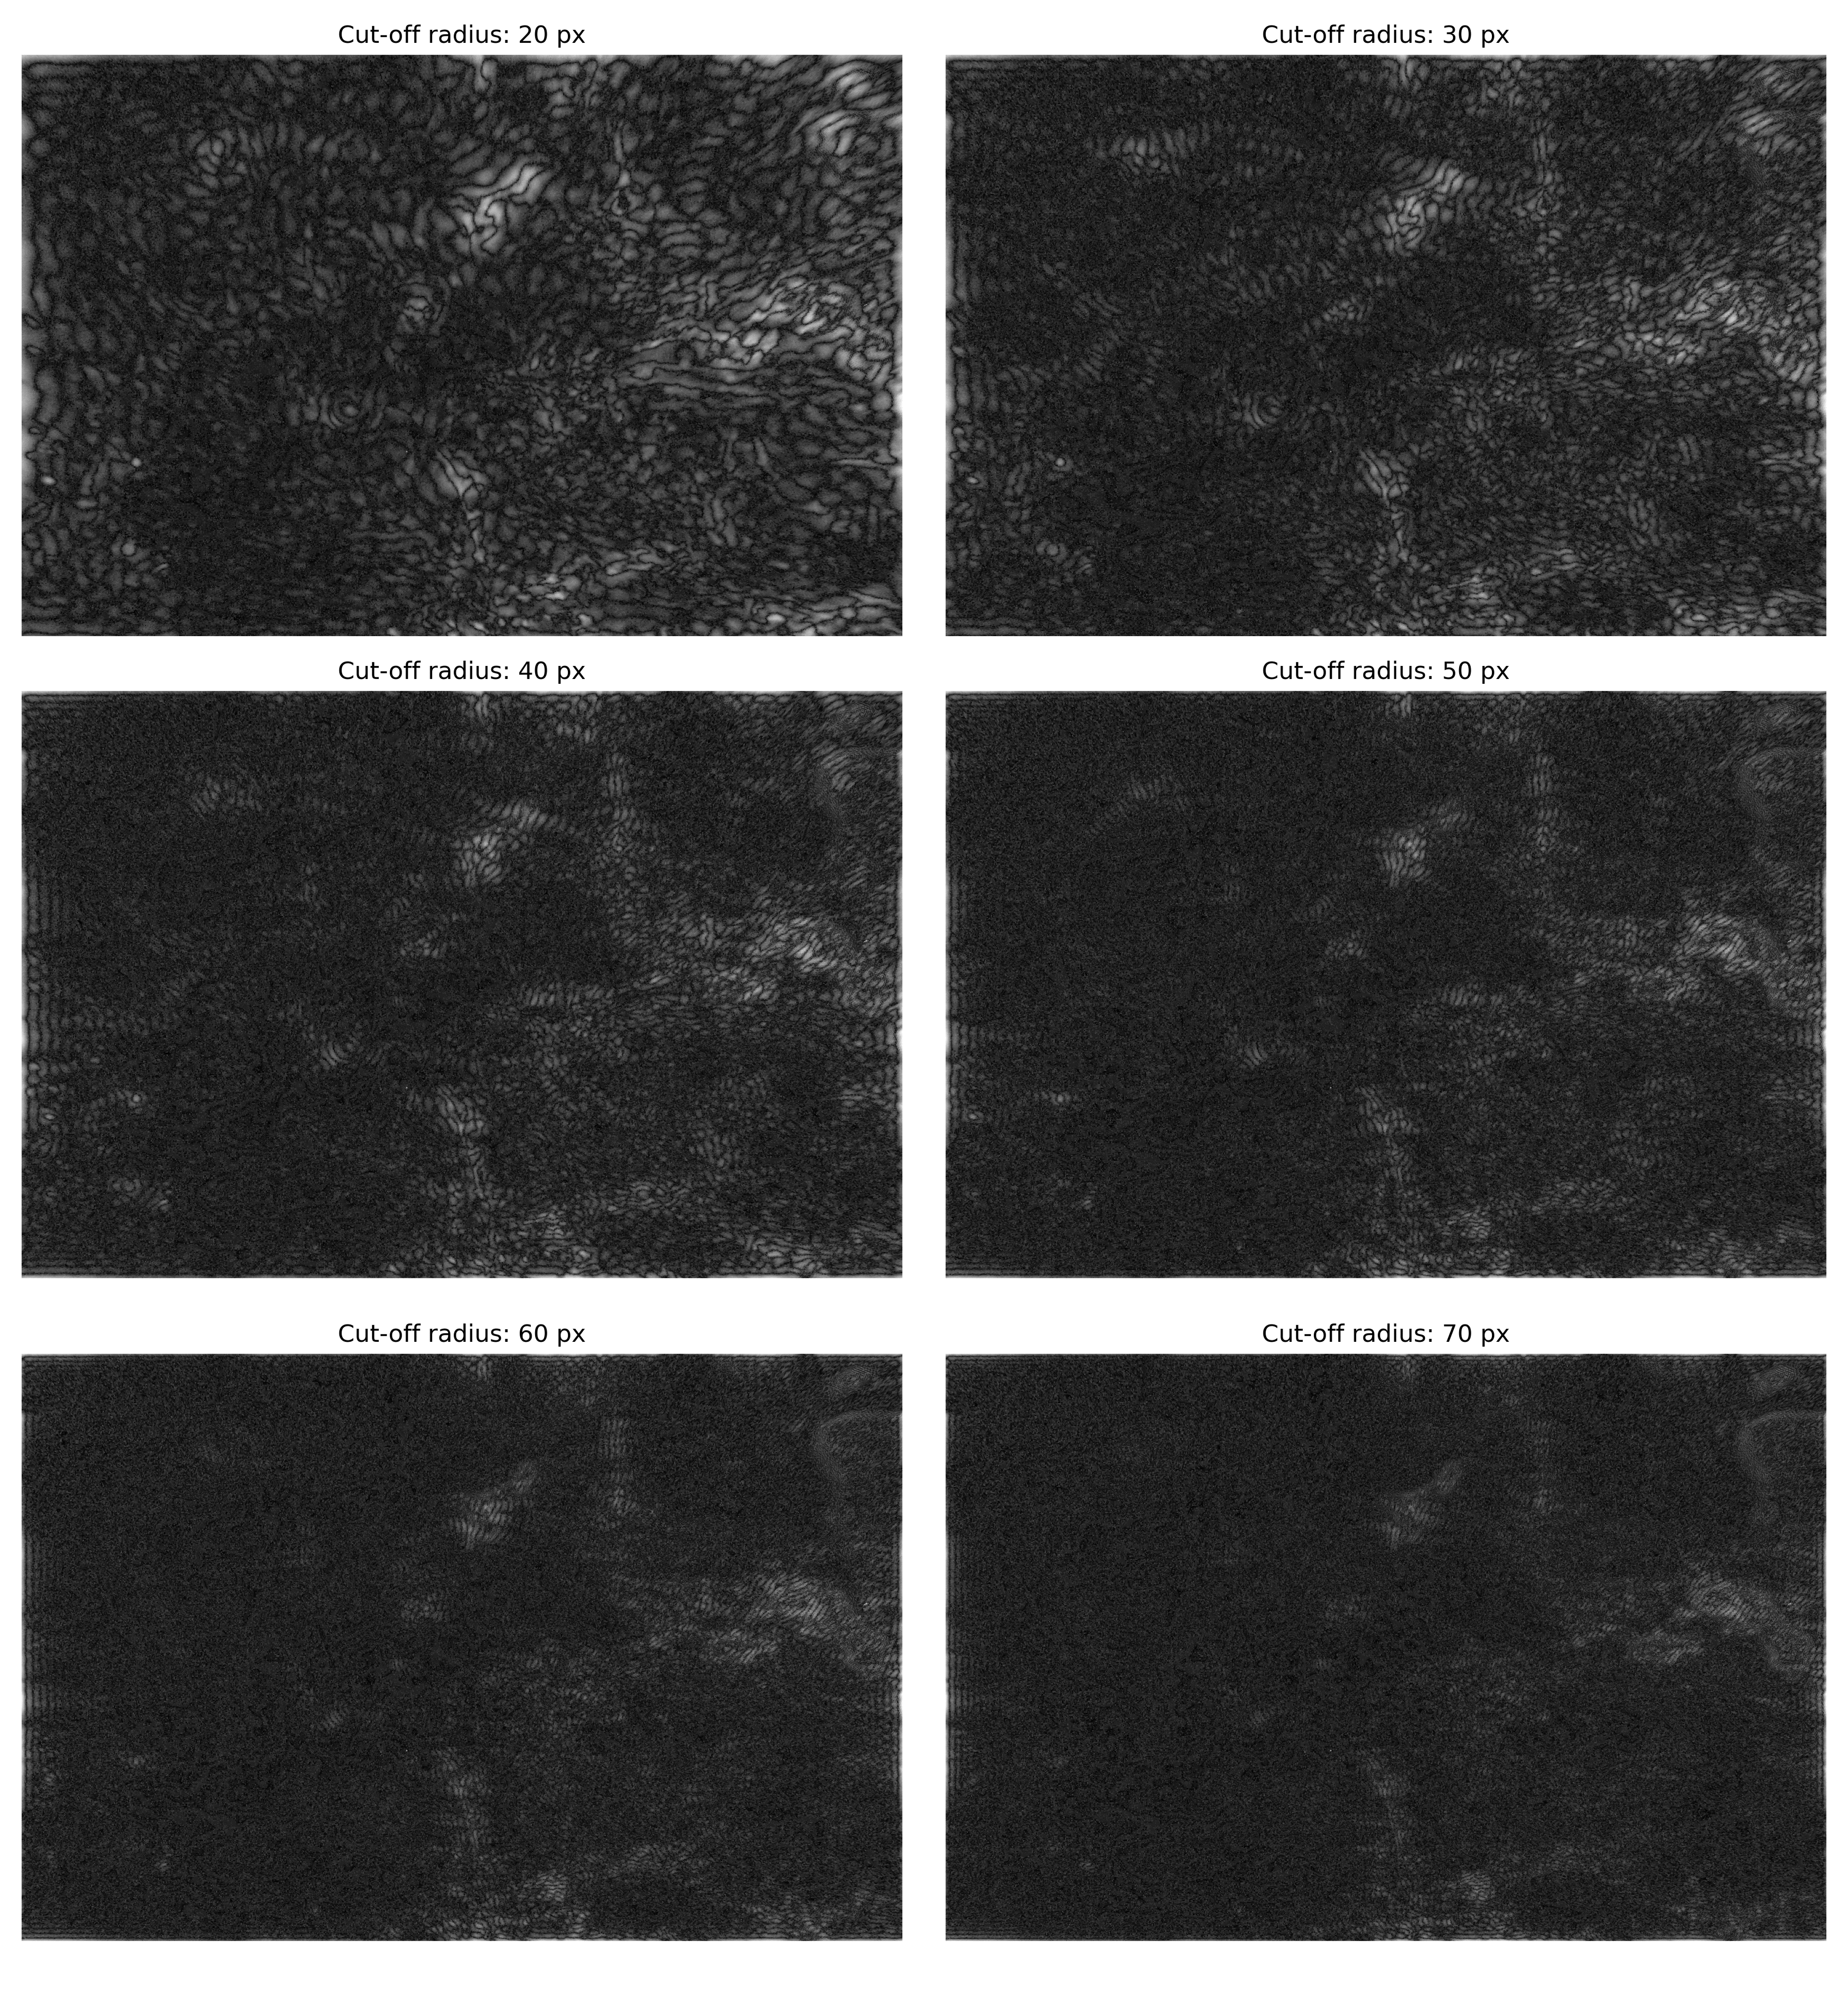
\includegraphics[width=0.9\textwidth]{appendix_a.png}
    \caption{First image of the image sequence from UTC: 24/12/2021 10:30:07. A high-pass filter was applied with different cut-off radii and the square root of pixel intensities was computed to enhance the result.}
\end{figure}
\FloatBarrier
\begin{figure}[h!]
    \centering
    \includegraphics[width=0.9\textwidth]{appendix_b.png}
    \caption{Meridional plots of each image sequence displaying the north-south direction component of wind speeds as a function of latitude.}
\end{figure}
\FloatBarrier
\begin{figure}[h!]
    \centering
    \includegraphics[width=0.9\textwidth]{appendix_c.png}
    \caption{Wind field results: UTC 22/11/2021 14:16:52 - 14:56:52}
\end{figure}
\FloatBarrier
\begin{figure}[h!]
    \centering
    \includegraphics[width=0.9\textwidth]{appendix_d.png}
    \caption{Wind field results: UTC 04/12/2021 00:31:53 - 01:11:53}
\end{figure}
\FloatBarrier
\begin{figure}[h!]
    \centering
    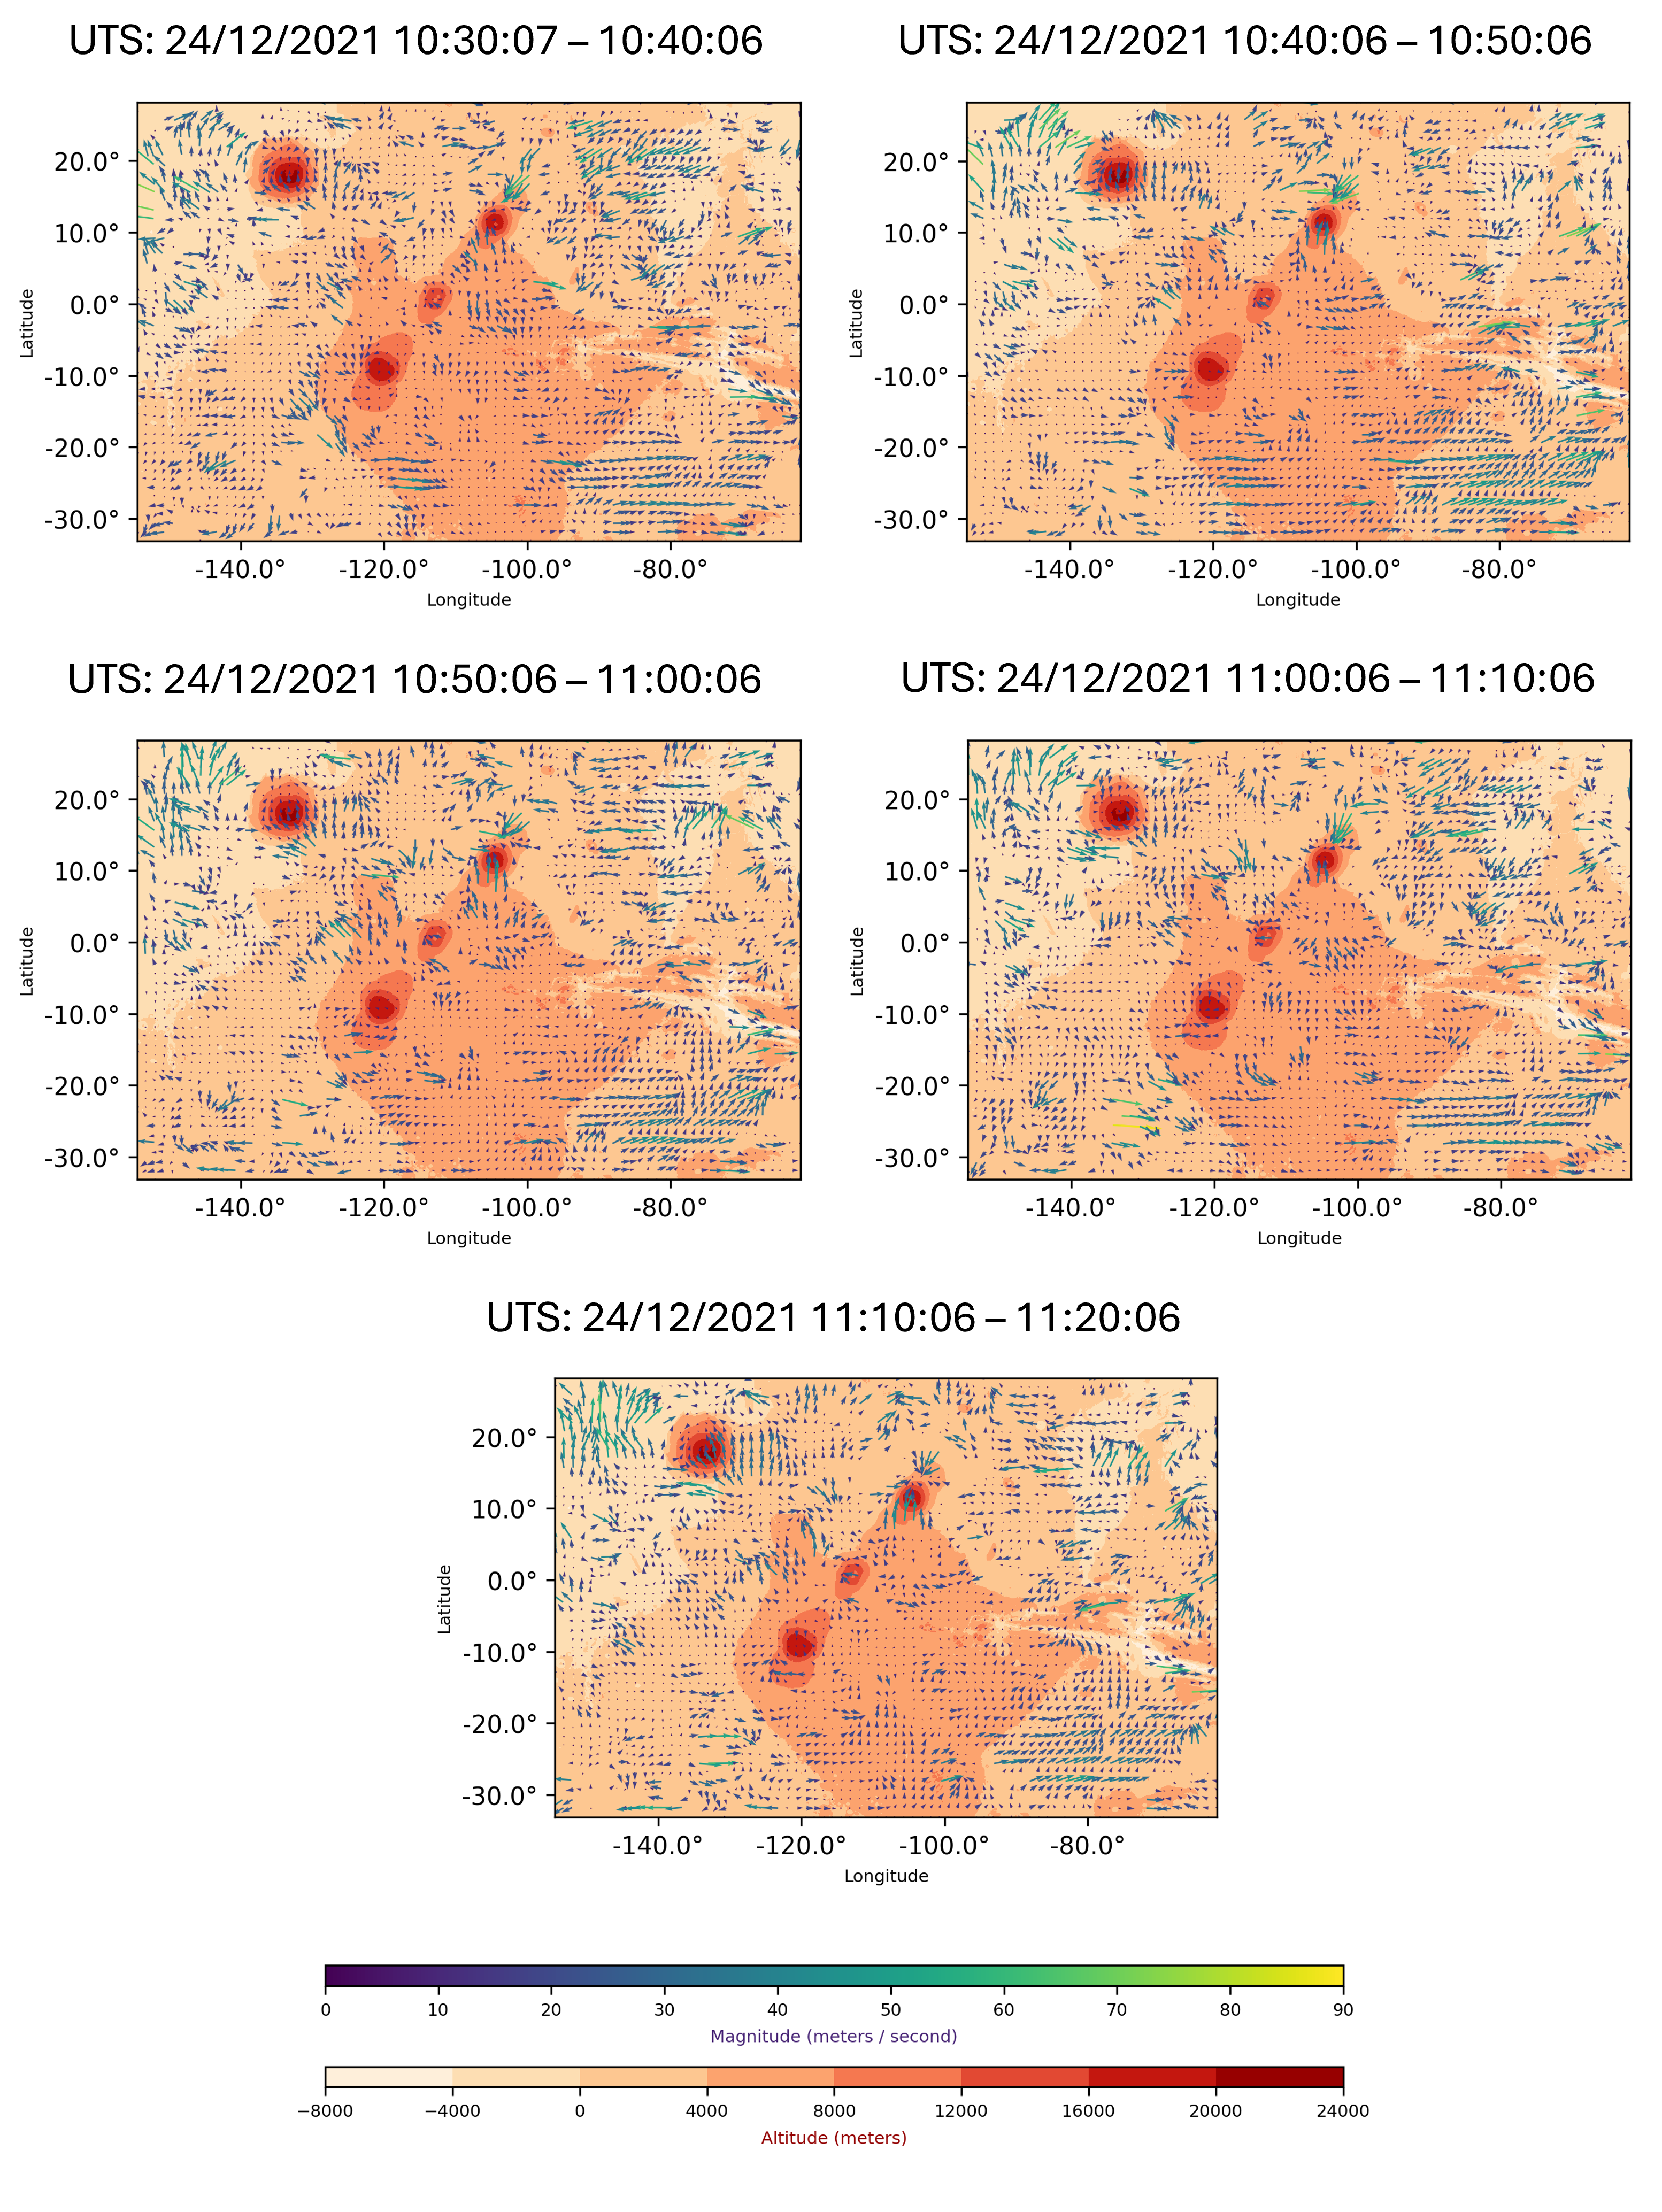
\includegraphics[width=0.9\textwidth]{appendix_e.png}
    \caption{Wind field results: UTC 24/12/2021 10:30:07 - 11:20:06}
\end{figure}
\FloatBarrier
\begin{figure}[h!]
    \centering
    \includegraphics[width=0.9\textwidth]{appendix_f.png}
    \caption{Wind field results: UTC 23/10/2023 05:40:13 - 06:40:19}
\end{figure}
\FloatBarrier
\begin{figure}[h!]
    \centering
    \includegraphics[width=0.9\textwidth]{appendix_g.png}
    \caption{Wind field results: UTC 23/10/2023 08:18:33 - 09:18:39}
\end{figure}
\FloatBarrier
\begin{figure}[h!]
    \centering
    \includegraphics[width=0.9\textwidth]{appendix_h.png}
    \caption{Wind field results: UTC 23/10/2023 10:56:50 - 11:56:56}
\end{figure}